\documentclass{article}
\usepackage[utf8]{inputenc}
\usepackage{amsmath}
\title{Report Lab 1: Radio Engineering}
\author{Henning Schei}
\date{March 2016}
\usepackage{natbib}
\usepackage{graphicx}
\usepackage{listings}
\usepackage{color}
\usepackage{float}
\definecolor{dkgreen}{rgb}{0,0.6,0}
\definecolor{gray}{rgb}{0.5,0.5,0.5}
\definecolor{mauve}{rgb}{0.58,0,0.82}

\lstset{frame=tb,
  language=Matlab,
  aboveskip=3mm,
  belowskip=3mm,
  showstringspaces=false,
  columns=flexible,
  basicstyle={\small\ttfamily},
  numbers=none,
  numberstyle=\tiny\color{gray},
  keywordstyle=\color{blue},
  commentstyle=\color{dkgreen},
  stringstyle=\color{mauve},
  breaklines=true,
  breakatwhitespace=true,
  tabsize=3
}
\begin{document}
\maketitle

\section{Task 1}

Since the lowest RX-sensitivity level is -97 dBm, the maximum reciever noise figure that will give a SNR of 0 dB is -97 dBm. 


\section{Task 2}
The figure[1] shows the difference between the horizontal and vertical polarization. The reason why the horizontal wave is stronger may be the fact that the vertical wave are beeing attenuated by the surface. Since sea is not a smooth surface, it will be scattered and attenuated. 
\begin{figure}[H]
  \centering
      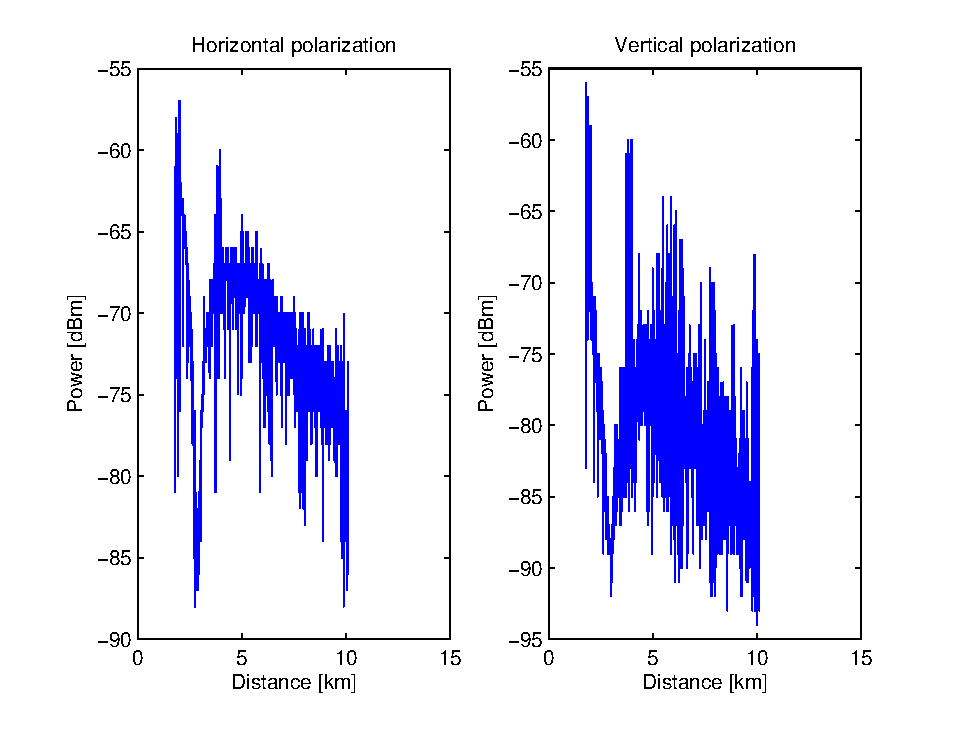
\includegraphics[width=0.85\textwidth]{task2.eps}
  \caption{Measurment data of vertical and horizontal polartization.}
\end{figure}
\section {Task 3}
The model does fit the data very well. The charactheristic dip in the curve are also very accurate
As the model approaches zero when the arguments in the sine and cosine apporaches 2*pi the mearsurement data does the same. 

\begin{figure}[H]
  \centering
      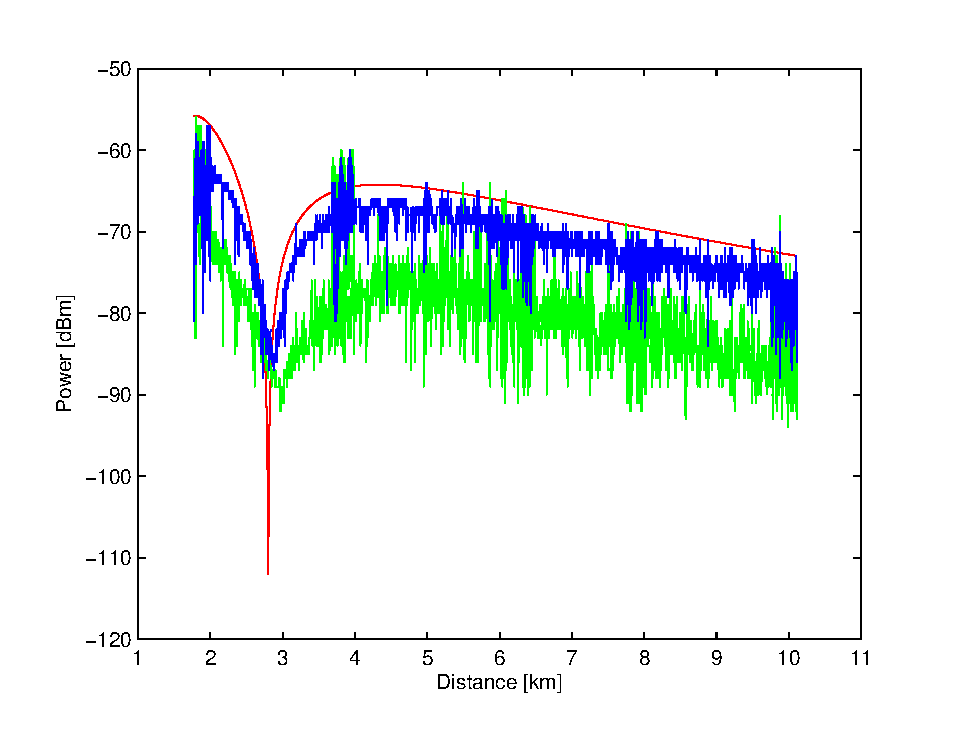
\includegraphics[width=1.0\textwidth]{task3.eps}
  \caption{Measurment data of vertical, horizontal polartization and the two path model from appendix. blue = horizontal, green = vertical}
\end{figure}


\section {Task 4}

The maximum range of a cell highest MCS $d = 3.6520e+04 $. xxx for lowest MCS


\begin{lstlisting}
% Assignment 1
% Henning Schei
close all;
clear all;

T  = 300; % Kelvin
Fc = 5.6e9; % Carrier frequency
%Bw = 60e6;  % System bandwidth
load('rssi_distance_omni_boat', '-mat')
% To obtain a SNR of 0 dB, the reciever must have a noise figure
% less than -97 dBm ? 



% Problem 2. 
subplot(1,2,1)
plot(d1, rssi1); 
xlabel 'Distance [km]'
ylabel 'Power [dBm]'
title 'Horizontal polarization'
subplot(1,2,2)
plot(d2,rssi2)
xlabel 'Distance [km]'
ylabel 'Power [dBm]'
title 'Vertical polarization'

figure;
plot(d1,power(rssi1/10,10));



% Problem 3.
c0  = 3e8;
d = d1;
lamb = Fc/c0; %meters
E1 = lamb/(4*pi); % in meters
E1_km  = E1*1000;

hTX = 25; hRX = 3; % 
d_phi = 2*hTX*hRX*2*pi*Fc ./ (d*1000*c0);
Etot = E1.* (1./(d.*1000)).* sqrt( power(1-cos(d_phi),2) + power(sin(d_phi),2));
figure;
plot(d,Etot);
Etot = 20*log10(Etot) ;
figure;
plot(d,Etot,'r'); hold on; plot(d2,rssi2,'g'); hold on; plot(d1,rssi1);

xlabel 'Distance [km]'
ylabel 'Power [dBm]'

% Problem 4
%-------------------------
% Lowest MCS (-97 dBm)
% Highest MCS (-74 dBm)

MCS_low  = -97-30 ; %db
MCS_high = -74 -30 ; %db

TX_power_dbm = 23; %dbm
TX_power_db  = TX_power_dbm -30 ; 
TX_gain_db = 23;%dbi
RX_gain_db = 12; %dbi

TX_gain = 10^(TX_gain_db/10);
RX_gain = 10^(RX_gain_db/10);
TX_power= 10^(TX_power_db/10);


PRX = TX_power * TX_gain * RX_gain * power((hTX*hRX./(power(d1,2))),2);
PRX_db = TX_power_db+ TX_gain_db + RX_gain_db  + 2*(log10((hTX*hRX)) - 2*log10(d1));



figure;
plot(d1,PRX_db)
hold on 
plot(d1, MCS_high);
plot(d1,MCS_low);


figure;
plot(d1*1000,PRX);
hold on;
plot(d1*1000, 10^(MCS_high/10));
hold on;
plot(d1*1000, 10^( MCS_low/10));

\end{lstlisting}






\end{document}



